\documentclass[preprint, 10pt]{elsarticle}

\newcommand{\mcaption}[2]{\caption{\small \em #1}\label{#2}}
\newcommand{\secref}[1]{\ref{#1}}

\usepackage{amsfonts}
\usepackage[fleqn,reqno]{amsmath}
\usepackage{amssymb}
\usepackage[titletoc]{appendix}
\usepackage{enumitem}
\usepackage{filecontents}
\usepackage[top=1.2in,bottom=1.2in,left=1in, right=1in]{geometry}
\usepackage{graphics}
\usepackage{lineno}
%\usepackage{showkeys} %To see the labels for now.  Will remove later
\usepackage{pgfplots}
\usepackage{tikz}
\usepackage{todonotes}

\usetikzlibrary{arrows}


%%%%%%  pdftex  %%%%%%%%%%%%%%%%%%%%%%%%%%%%%%%%%%%%%%%%%%%%%%%%%%%%%%
\usepackage[pagebackref=false,bookmarks=false]{hyperref} 

\hypersetup{
  bookmarksnumbered=true,
  bookmarksopen=false,
  hypertexnames=false,      
  breaklinks=true,          
  unicode=false,
  pdffitwindow=true,        
  pdfnewwindow=true,        
  colorlinks=true,         
  linkcolor=dblue,
  anchorcolor=red,
  citecolor=dorange,
  filecolor=magenta,
  urlcolor=dblue,
  pdfstartview = FitH,
  pdfkeywords = {},
  pdfcreator = {LaTeX with hyperref package}
}

\newcommand{\bd}{{\partial}}
\newcommand{\cc}{{\mathbf{c}}}
\newcommand{\DD}{{\mathcal{D}}}
\newcommand{\eeta}{{\boldsymbol\eta}}
\newcommand{\ff}{{\mathbf{f}}}
\newcommand{\grad}{{\nabla}}
\newcommand{\llambda}{{\boldsymbol\lambda}}
\newcommand{\nn}{{\mathbf{n}}}
\newcommand{\NN}{{\mathcal{N}}}
\newcommand{\pderiv}[2]{\frac{\partial #1}{\partial #2}}
\newcommand{\rr}{{\mathbf{r}}}
\newcommand{\RR}{{\mathbb{R}}}
\renewcommand{\ss}{{\mathbf{s}}}
\newcommand{\ssigma}{{\boldsymbol\sigma}}
\newcommand{\uu}{{\mathbf{u}}}
\newcommand{\UU}{{\mathbf{U}}}
\newcommand{\vv}{{\mathbf{v}}}
\newcommand{\xx}{{\mathbf{x}}}
\newcommand{\xxi}{{\boldsymbol{\xi}}}
\newcommand{\yy}{{\mathbf{y}}}

\begin{document}

\title{Methods paper for rigid bodies}

\author[Lukas]{Lukas Bystircky}
\author[Lukas]{Sachin Shanbhag}
\author[Bryan]{Bryan D.~Quaife}
\address[Lukas]{Department of Scientific Computing, Florida State University, Tallahassee, FL, 32306.}
\address[Bryan]{Department of Scientific Computing and Geophysical Fluid Dynamics Institute, Florida State University, Tallahassee, FL, 32306.}

\begin{abstract} 
We consider suspensions of rigid bodies in two dimensions \ldots
\end{abstract}

\begin{keyword}
  Stokes flow \sep Boundary integral method \sep Rigid body suspensions 
\end{keyword}

\maketitle





%%%%%%%%%%%%%%%%%%%%%%%%%%%%%%%%%%%%%%%%%%%%%%%%%%%%%%%%%%%%%%%%%%%%%%%
\section{Introduction\label{s:intro}}

\todo[inline]{Bryan will write this section}

This is a methods paper
\begin{itemize}
  \item Boundary integral equation formulation
  \item STIV
  \item FMM
  \item Near-singular integration
  \item Pressure and energy dissipation calculations
  \item Time integrator
\end{itemize}




%%%%%%%%%%%%%%%%%%%%%%%%%%%%%%%%%%%%%%%%%%%%%%%%%%%%%%%%%%%%%%%%%%%%%%%
\section{Formulation\label{s:formulation}} 

\subsection{Problem Formulation}

We will consider a collection of particles in a planar (two dimensional) flow. The fluid will be in a domain $\Omega$ with a boundary $\partial\Omega$. The boundary $\partial\Omega$ is the union of the surfaces of $N$ suspended particles each with a boundary $\Gamma_k$, $1\leq k \leq N$, the surfaces of $M$ solid walls each with boundary, $\Gamma_\ell$ $N+1\leq\ell\leq N+ M$ and optionally a containing wall  denoted $\Gamma_0$. The suspended particles are all rigid and at each time step we will solve for their translational velocity $\mathbf{u}^{\tau}_k$ and angular velocity $\omega_k$, allowing us to update their centers and orientations, $\mathbf{c}_k$ and $\theta_k$ respectively. Particles and interior walls will be undergoing a net force $\mathbf{F}_{k/\ell}$  and torque $L_{k/\ell}$. 

\begin{figure}[!h]
\begin{center}
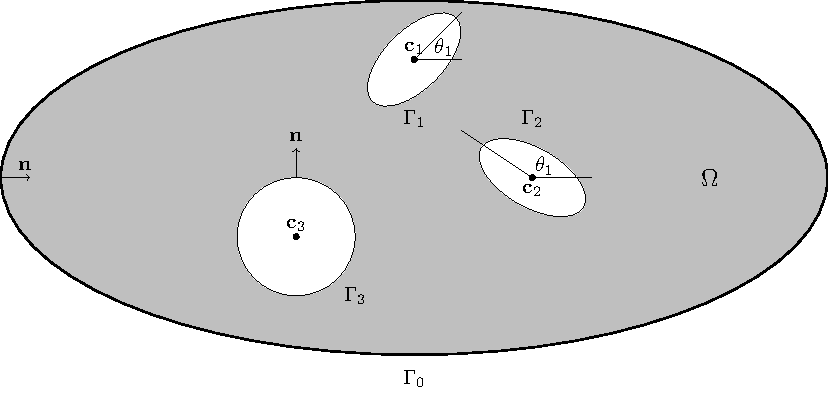
\includegraphics{figures/multiply_connected.pdf}
\end{center}
\caption{Sketch of a possible domain $\Omega$. $\Gamma_1$ and $\Gamma_2$ enclose particles, while $\Gamma_3$ encloses a solid wall. The outer boundary $\Gamma_0$ need not be present. The boundary $\partial\Omega$ is $\Gamma_0\cup\bigcup\limits_{i=1}^{N+M}\Gamma_i$. The vector $\mathbf{n}$ is the unit normal vector pointing into the fluid domain. }
\end{figure}
\subsection{Repulsion Forces}

\begin{figure}[!h]\label{fig:collision_sketch}
\begin{center}
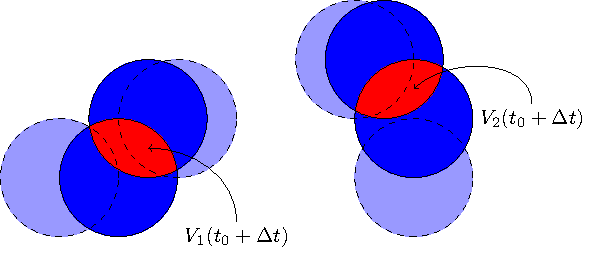
\includegraphics{figures/collisions.pdf}
\end{center}
\caption{Sketch of potential collisions.}
\end{figure}
It is well known that the exact solutions of the Stokes equations prohibit contact between particles in finite time due to lubrication forces. In theory therefore if we solve the Stokes equations accurately enough contact will be avoided. Achieving this level of accuracy however could require a prohibitively fine mesh or small time step size, in particular for dense suspensions. In order to keep computational costs reasonable we must turn to alternative approaches. 

One such approach is to introduce an artificial repulsion force. There are many possible choices for the type of force. One possibility is a Leonard-Jones type force that grows exponentially as two particles become close together (need citations). This has been shown to work for dense suspensions, however the resulting ODEs become very stiff as the separation between particles decreases, thus requiring smaller time steps. In addition this type of force does guarantee no collisions. If the time step is too large collisions can still occur. An alternative approach is to choose the forces in such a way as to explicitly guarantee each time step is collision free. 

The main algorithm will proceed as follows. At each time step $t^n$ the Stokes equations are solved and the particles are advanced to a candidate configuration at $t^{n+1}$. At this point we can check for collisions. If no collisions are found, the candidate configuration is accepted, otherwise it is rejected and we resolve the Stokes equations at $t^n$ with an artificial repulsion force, adjusting this force as necessary until the candidate configuration at time $t^{n+1}$ is collision free and can be accepted. The remainder of this section is dedicated to describing how this artificial repulsion force is computed. 


\subsection{Contact definition}

Before any discussion of resolving collisions we must define a metric that measures collisions. This metric will keep track of all possible pairwise collisions. If an entry of $\mathbf{V}(t)$ is less than 0 at a time $t$, then a collision has occurred and a repulsion force must be added. There are several possible choices for $\mathbf{V}(t)$, the simplest of which is simply a signed distance between all points on all particles. We will use the concept of \textit{Space-Time Interference Volumes} (STIV) introduced by Harmon et al.\cite{Harmon2011} and adapted for suspension modeling by Lu et al.\cite{Lu2017}. 

Given a particle configuration $S(t)$ for which $S(t_0)$ is collision-free, for each point $\mathbf{X}(s,t)$ on $S(t)$ we define $\tau_I(s)$, $t_0 < \tau_I \leq t$ to be the first instance for which $\mathbf{X}$ comes into contact with a different point on $S(t)$. The STIV for the time interval $[t_0, t]$ is 
\[ V(S, t) = -\int_{S(t_0)}\int_{\tau_I(s)}^t \sqrt{\epsilon^2 + (\mathbf{u}(s, \tau)\cdot\mathbf{n}(s,\tau))^2}~\text{d}\tau\text{d}s,\]
where the constant $\epsilon$ is a smoothing parameter. The time integral in this expression ensures that no contact is missed even if one particle passes completely through another (or through a solid wall) in a single time step. This allows us to take large time steps and not be worried about missing collisions. $\mathbf{V}(S,t)$ can be interpreted as the area of the surface with coordinate $(\mathbf{X}(s,\tau),\epsilon\tau)$ for all $(s,\tau)$ such that $\tau_I(s)\leq t$. 

In \cite{Lu2017} an infinitesimal version of the STIV is derived. Starting from a collision-free configuration at $t_0$, for a fixed $\tau$ the set of points $s$ such that $\tau_I(s)\leq \tau$ is the contact area. This area is a set of boundary segments. For one such segment we can let $s_1(\tau)$ and $s_2(\tau)$ be the extents of contact at time $\tau$. 

\[ \mathbf{V}(\mathbf{u},t) = -\int_{s_1(t)}^{s_2(t)} \sqrt{\epsilon^2 + (\mathbf{u}(s,t)\cdot\mathbf{n}(s,t))^2}\text{d}s + \epsilon,\]
along with the variation, 
\[ \text{d}_{\mathbf{u}}V[\delta\mathbf{u}] = -\int_{s_1(t)}^{s_2(t)}\frac{(\mathbf{n}\cdot\mathbf{u})(\mathbf{n}\cdot\delta\mathbf{u})}{\sqrt{\epsilon^2 + (\mathbf{u}\cdot\mathbf{n})^2}}\text{d}s.\]


\subsection{Governing Equations}\label{sec:governing}
The governing equations for this problem are the incompressible Stokes equations,
\begin{subequations}\label{eq:stokes}
\begin{align}
	-\mu\Delta \mathbf{u} + \nabla p &= \mathbf{f} \text{ in }\Omega,\\
	\nabla\cdot\mathbf{u} &= 0 \text{ in }\Omega,
\end{align}
\end{subequations}
where $\mathbf{u}(\mathbf{x})$ is the fluid velocity, $p(\mathbf{x})$ is the fluid pressure, $\mathbf{f}(\mathbf{x})$ are body forces acting on the fluid and $\mu$ is the dynamic viscosity of the fluid. For simplicity we will take $\mu$ to be 1 for the remainder of this paper. We will assume Dirichlet boundary conditions on the velocity,
\begin{equation}\label{eq:boundary_condition}
	 \mathbf{u} = \mathbf{u}_b \text{ on } \partial\Omega,\end{equation}
subject to the constraint 
\begin{equation}\label{eq:compatibility}
	 \int_{\Gamma_i} \mathbf{u}_b\cdot\mathbf{n}~\text{d}s = 0, \qquad 0\leq i \leq N+M,
\end{equation}
which is necessary for global conservation of mass and does not allow for sources or sinks.

The incompressible Stokes equations can be can be restated as a minimization problem. Consider the functional,
\[ \mathcal{J}(\mathbf{u}) = \int_{\Omega} \nabla\mathbf{u}:\nabla\mathbf{u} - 2\mathbf{f}\cdot\mathbf{u} ~\text{d}\Omega,\]
and the associated constrained minimization problem,
\[ \min \mathcal{J}(\mathbf{u}) ~:~ \nabla\cdot\mathbf{u} = 0 \text{ in }\Omega.\]
Introducing $p$, a Lagrange multiplier for the incompressibility condition, we can construct a Lagrangian for this system,
\begin{equation}\label{eq:lagrangian} \mathcal{L}(\mathbf{u},p) = \mathcal{J}(\mathbf{u}) - \int_{\Omega} 2p\nabla\cdot\mathbf{u}~\text{d}\Omega.\end{equation}
First order optimality (KKT) conditions for $\mathcal{L}(\mathbf{u},p)$ recover the incompressible Stokes equations. For our problem, in addition to the incompressibility condition, we wish to enforce the constraint that the solution $\mathbf{u}$ at a time $t_0$ should not introduce collisions at time $t_0+\Delta t$, in other words $\mathbf{V}(t_0 + \Delta t) \geq \mathbf{0}$.
This constraint can be incorporated in the Lagrangian \eqref{eq:lagrangian} with the introduction of a Lagrange multiplier $\pmb{\lambda}$ with one component for each possible collision volume,
\begin{equation}\label{eq:lagrangian2} \tilde{\mathcal{L}}(\mathbf{u},p,\lambda) = \mathcal{L}(\mathbf{u},p) + \pmb{\lambda} \cdot \mathbf{V}(t_0+\Delta t).\end{equation}
First order optimality for \eqref{eq:lagrangian2} yields the Stokes equations with a modified forcing function,
\begin{equation}\label{eq:stokes_mod}-\Delta \mathbf{u} + \nabla p = \mathbf{f} + \int_{\Omega} \text{d}_{\mathbf{u}} \mathbf{V}^T\pmb{\lambda} ~\text{d}\Omega,\end{equation}
subject to the constraints
\[\nabla\cdot\mathbf{u}  =0, ~\mathbf{V}(t_0 + \Delta t) \geq 0,~\pmb{\lambda} \geq 0, ~ \pmb{\lambda}\cdot\mathbf{V}(t_0+\Delta t) = 0.	\]

\subsection{Complementary Problem}

Given a configuration $\mathbf{q}^n$ at $t_n$ we can solve for the velocity without any repulsion $\mathbf{u}^*$ by solving the system,
\[ \mathbf{u}^* = \mathbf{A}(\mathbf{q}^n),\]
where $\mathbf{A}(\mathbf{q}^n)$ is some linear system arising from a discretization of the Stokes equations. To include the contributions to the velocity from the Stokes equations we can add an additional term,
\[ \mathbf{u} = \mathbf{u}^* + \pmb{\lambda} \mathbf{B} \mathbf{f}_c,\]
Where $\mathbf{B}$ is some linear mapping from the repulsion force $\pmb{\lambda}\mathbf{f}_c$ to an induced velocity. Once we have the velocity the configuration can be updated using an explicit Euler step,
\[ \mathbf{q}^{n+1} = \mathbf{q}^n + \Delta t\mathbf{u}^n.\]

The complementary conditions can be stated as
\[ \mathbf{V}(\mathbf{q}^n,\mathbf{u}) \geq 0 \perp \pmb{\lambda} \geq 0.\]
Since $\mathbf{u}$ depends on $\pmb{\lambda}$, so does $\mathbf{V}$ and in general this relationship is nonlinear. To linearize this constraint we can use a first order Taylor series expansion of $\mathbf{V}$ to get
\[ \mathbf{V}(\mathbf{q}^n,\mathbf{u}) = \mathbf{V}(\mathbf{q}^n,\mathbf{u}^* + \lambda \mathbf{B} \mathbf{f}_c) \approx \mathbf{V}(\mathbf{q}^n,\mathbf{u}^*) + \text{d}_\mathbf{u}\mathbf{V}(\mathbf{q}^n,\mathbf{u}^*)\cdot\mathbf{B}\mathbf{f}_c\pmb{\lambda}.\]
This gives us a linear complementary problem, which we can solve for $\pmb{\lambda}$,
\[ \mathbf{V}(\mathbf{q}^n,\mathbf{u}^*) + \text{d}_\mathbf{u}\mathbf{V}(\mathbf{q}^n,\mathbf{u}^*)\cdot\mathbf{B}\mathbf{f}_c\pmb{\lambda} \geq 0 \perp \pmb{\lambda} \geq \ 0.\]



\subsection{Boundary Integral Equation Representation}

As discussed in section \ref{sec:governing}, the governing equations for this problem are the incompressible Stokes equations. There are many ways to solve these equations, here we will use \textit{boundary integral equations} (BIEs). For the Stokes BIEs have many advantages over other numerical methods such as finite element or finite volume methods. A discussion of the benefits of BIEs for this problem can be found in \cite{Karrila1989}. 

\subsubsection{Unbounded Domains}

In an unbounded domain there will be an imposed background flow $\mathbf{u}_{\infty}$. We will use BIEs to solve for a velocity perturbation $\mathbf{u}_p$ due to the boundary conditions on particles and solid walls.

The solution to the Stokes equations \eqref{eq:stokes} with a homogeneous forcing function at a point $\mathbf{x}$ inside a domain $\Omega$ can be expressed as an integral around the boundary of the domain $\partial\Omega$,
\begin{equation}\label{eq:dlp}\mathbf{u}_p(\mathbf{x}) = \mathcal{D}[\pmb{\eta}](\mathbf{x}) = \frac{1}{\pi}\int_{\partial\Omega} \frac{\mathbf{r}\cdot\mathbf{n}}{\rho^2}\frac{\mathbf{r}\otimes\mathbf{r}}{\rho^2}\pmb{\eta}(\mathbf{y})~\text{d}s(\mathbf{y}),\end{equation}
where $\pmb{\eta}$ is an unknown density function defined only along $\partial\Omega$, $\mathbf{r}=\mathbf{x}-\mathbf{y}$ and $\rho=|\mathbf{r}|$. The operator $\mathcal{D}[\pmb{\eta}]$ is the double layer potential and can be derived from the fundamental solution of \eqref{eq:stokes} \cite{Ladyzhenskaya1963, Pozrikidis1992}. The double layer potential by itself cannot represent all possible flow fields. In particular it cannot represent flows around surfaces undergoing a net force or torque. Following \cite{Power1987, Power1993} for surfaces undergoing an arbitrary net force $\mathbf{F}$ and net torque $L$ we can complete the double layer potential as,
\[ \mathbf{u}(\mathbf{x}) = \mathbf{u}_{\infty} +  \mathcal{D}[\pmb{\eta}] + \sum\limits_{i=1}^{N+M} \left(\mathbf{S}(\mathbf{x},\mathbf{c}_i)\mathbf{F}_i + \mathbf{R}(\mathbf{x},\mathbf{c}_i)L_i\right),\]
where the Stokeslet $\mathbf{S}(\mathbf{x},\mathbf{y})$ and rotlet $\mathbf{R}(\mathbf{x},\mathbf{y})$ are given by
\[ \mathbf{S}(\mathbf{x},\mathbf{y}) = \frac{\mathbf{r}\otimes\mathbf{r}}{\rho^2} - \log\rho\mathbf{I},\qquad \mathbf{R}(\mathbf{x},\mathbf{y}) = \frac{\mathbf{r}^\perp}{\rho^2}.\]
Note that we have also added back in the background flow.

 To set up a system to solve we can take the limit of \eqref{eq:dlp} as we approach $\partial\Omega$ and match it to the boundary condition \eqref{eq:boundary_condition}. The double layer potential is not continuous when we cross the boundary and has a limiting value of $-\pmb{\eta}/2$. This leads to the second kind Fredholm equation,
\begin{equation}\label{eq:vel_walls} -\frac{1}{2}\pmb{\eta}(\mathbf{x}) + \mathcal{D}[\pmb{\eta}](\mathbf{x}) + \sum\limits_{i=1}^{N+M} \left(\mathbf{S}(\mathbf{x},\mathbf{c}_i)\mathbf{F}_i + \mathbf{R}(\mathbf{x},\mathbf{c}_i)L_i\right) = \mathbf{u}_b - \mathbf{u}_\infty.\end{equation}

On solid walls we will prescribe the velocity $\mathbf{u}_b$ and solve for the net force and torque on each wall. This is called the \textit{resistance problem}. For particles on the other hand we will prescribe the net force and torque on each particle and solve for the velocity $\mathbf{u}_b$. This is known as the \textit{mobility problem}. We will use the fact that the particles are rigid to decompose $\mathbf{u}_b$ into a translational and rotational component,
\[ \mathbf{u}_b = \mathbf{u}^\tau + \omega(\mathbf{x}-\mathbf{c})^\perp.\]
This lets us set up an equation to solve for the velocity on the surface of particle $k$,
\begin{equation}\label{eq:vel_particles} -\frac{1}{2}\pmb{\eta}(\mathbf{x}) + \mathcal{D}[\pmb{\eta}](\mathbf{x}) - \mathbf{u}^\tau_k - \omega(\mathbf{x}-\mathbf{c}_k)^\perp =  -\sum\limits_{i=1}^{N+M} \left(\mathbf{S}(\mathbf{x},\mathbf{c}_i)\mathbf{F}_i + \mathbf{R}(\mathbf{x},\mathbf{c}_i)L_i\right) - \mathbf{u}_\infty.\end{equation}

For the both the resistance and mobility problem we have more unknowns than equations. In particular, we have to solve for two components of $\pmb{\eta}$ and either 
\begin{enumerate}[label=(\alph*)]
	\item two components of net force and a net torque for each solid wall $\rightarrow$ an additional $3M$ unknowns
	\item two components of translational velocity and an angular velocity of each particle $\rightarrow$ an additional $3N$ unknowns
\end{enumerate}

To close these systems we will follow \cite{Power1993} and relate $\pmb{\eta}$ to the net force and torque on each particle or wall. In particular for $1\leq i \leq N+M$,
\begin{subequations}\label{eq:closure}
\begin{align}
	&\int_{\Gamma_i} \pmb{\eta}~\text{d}s = \mathbf{F}_i,\\
	&\int_{\Gamma_i} \pmb{\eta}\cdot (\mathbf{x} - \mathbf{c})^\perp~\text{d}s = L_i.
\end{align} 
\end{subequations}

Combining \eqref{eq:vel_walls}, \eqref{eq:vel_particles} and \eqref{eq:closure} we can write our problem in the compact notation,
\begin{equation}\label{eq:stokes_unbounded} \begin{bmatrix} -\frac{1}{2} + \mathcal{D} & 1 & (\mathbf{x}-\mathbf{c})^\perp & \mathcal{S} & \mathcal{R}\\
		\int \cdot~ \text{d}s & 0 & 0 & 0 & 0\\
		\int\cdot(\mathbf{x}-\mathbf{c})^\perp~\text{d}s & 0 & 0 & 0 & 0\\
		\int \cdot~ \text{d}s & 0 & 0 & - 1 & 0\\
		\int\cdot(\mathbf{x}-\mathbf{c})^\perp~\text{d}s & 0 & 0 & 0 & -1\end{bmatrix}
\begin{bmatrix}
	\pmb{\eta}\\\mathbf{u}^\tau \\ \pmb{\omega} \\ \mathbf{F}_w \\\mathbf{ L}_w
\end{bmatrix}
=
\begin{bmatrix}
	-\mathbf{u}_{\infty} - \mathcal{S}\mathbf{F}_p - \mathcal{R}\mathbf{L}_p\\
	\mathbf{F}_p\\
	\mathbf{L}_p\\
	0\\
	0
\end{bmatrix}
\end{equation}

\subsubsection{Bounded Domains}

Bounded domains lead to a similar system, however it must be modified slightly. For fluid inside a container the double layer potential has a rank one null space \cite{Ladyzhenskaya1963}. Following \cite{Power1993} this null space can be removed by adding an operator that is active only over the enclosing boundary $\Gamma_0$,
\[ \mathcal{N}_0[\pmb{\eta}](\mathbf{x}) = \delta_{i0} \int_{\Gamma_i}\mathbf{n}(\mathbf{x})\otimes\mathbf{n}(\mathbf{y})~\text{d}s(\mathbf{y}).\]
The compatibility condition \eqref{eq:compatibility} ensures that this term evaluates to 0. Adding $\mathcal{N}_0$ to \eqref{eq:stokes_unbounded} and removing the background flow leads to the linear system,
\begin{equation}\label{eq:stokes_bounded} \begin{bmatrix} -\frac{1}{2} + \mathcal{D} + \mathcal{N}_0 & 1 & (\mathbf{x}-\mathbf{c})^\perp & \mathcal{S} & \mathcal{R}\\
		\int \cdot~ \text{d}s & 0 & 0 & 0 & 0\\
		\int\cdot(\mathbf{x}-\mathbf{c})^\perp~\text{d}s & 0 & 0 & 0 & 0\\
		\int \cdot~ \text{d}s & 0 & 0 & - 1 & 0\\
		\int\cdot(\mathbf{x}-\mathbf{c})^\perp~\text{d}s & 0 & 0 & 0 & -1\end{bmatrix}
\begin{bmatrix}
	\pmb{\eta}\\\mathbf{u}^\tau \\ \pmb{\omega} \\ \mathbf{F}_w \\\mathbf{ L}_w
\end{bmatrix}
=
\begin{bmatrix}
	 - \mathcal{S}\mathbf{F}_p - \mathcal{R}\mathbf{L}_p\\
	\mathbf{F}_p\\
	\mathbf{L}_p\\
	0\\
	0
\end{bmatrix}
\end{equation}

\subsection{Incorporating Repulsion Forces}

The addition of a forcing term to the right hand side of the Stokes equations would normally lead to a volume integral. However, in this case since $\text{d}_{\mathbf{u}} V$ can be non-zero only on the boundary, we can capture the repulsion force by adding a net force and torque to each particle or wall as needed. The net force $\mathbf{F}^k_p$ and torque $L^k_p$ are given by,
\[ \mathbf{F}^k_p = \int_{\Gamma_k} \text{d}_\mathbf{u}V^T\pmb{\lambda}~\text{d}s, \qquad L_p^k = \int_{\Gamma_k}  \text{d}_\mathbf{u}V^T\pmb{\lambda}\cdot(\mathbf{x}-\mathbf{c}_k)^\perp~\text{d}s.\]
		
%%%%%%%%%%%%%%%%%%%%%%%%%%%%%%%%%%%%%%%%%%%%%%%%%%%%%%%%%%%%%%%%%%%%%%%
\section{Numerical Methods\label{s:method}} 

The linear system \eqref{eq:stokes_unbounded} or \eqref{eq:stokes_bounded} is discretized using a collocation trapezoid method. For particles that are in near-contact the near singular integration scheme described in \cite{Quaife2014, Ying2006} is used. The discretized system is solved with GRMES \cite{Saad1986} with a block diagonal preconditioner and accelerated using the fast multipole method \cite{Greengard1987}.  Since the linear system arises from a second kind Fredholm equation the condition number of the matrix is bounded and does not increase with finer resolution. The number of GMRES iterations is therefore mesh resolution independent. This leads to a solver that is $O(n)$, where $n$ is the number of mesh points. 

Once we solve for the translational and angular velocity of the particles, the position and angle of each particle are updated according to the ODEs,
\[ \frac{\text{d}}{\text{d}t}\mathbf{c}_k = \mathbf{u}^\tau_k, \qquad \frac{\text{d}}{\text{d}t}\theta_k =\omega_k.\]
The ODEs are advanced in time using an explicit Euler step. 

The matrices described in \eqref{eq:stokes_unbounded} and \eqref{eq:stokes_bounded} are full. They can be made block-diagonal by treating inter-particle interactions explicitly and moving them to the right hand side. This is termed \textit{locally implicit} and is described in \cite{Lu2017}. For dense suspensions however this type of time stepping can lead to instabilities as particles become tightly packed. 

%%%%%%%%%%%%%%%%%%%%%%%%%%%%%%%%%%%%%%%%%%%%%%%%%%%%%%%%%%%%%%%%%%%%%%%
\section{Results\label{s:results}} 

\begin{itemize}
  \item One of the main results is that the new time integrator can
    handle higher concentrations
  \item Two bodies in extensional
  \item Multiple bodies in extensional and/or Taylor-Green
  \item Couette with low and high concentration
\end{itemize}

%%%%%%%%%%%%%%%%%%%%%%%%%%%%%%%%%%%%%%%%%%%%%%%%%%%%%%%%%%%%%%%%%%%%%%%
\section{Conclusions\label{s:conclusions}}


%%%%%%%%%%%%%%%%%%%%%%%%%%%%%%%%%%%%%%%%%%%%%%%%%%%%%%%%%%%%%%%%%%%%%%%
\begin{appendices}
An appendix
\end{appendices}


\bibliographystyle{plainnat} 
\bibliography{bibliography}
\biboptions{sort&compress}
\end{document}
